\documentclass[11pt]{article}
\usepackage{amsmath,amssymb,amsthm,mathtools}
\usepackage[margin=1in]{geometry}
\usepackage{algorithm}
\usepackage{algpseudocode}
\usepackage{xcolor}
\usepackage{graphicx}
\usepackage{booktabs,tabularx,array}
\usepackage{enumitem}
\usepackage[font=small,labelfont=bf]{caption}
\usepackage{microtype}
\usepackage[section]{placeins}
\usepackage[colorlinks=true,linkcolor=blue!50!black,citecolor=blue!50!black,urlcolor=blue!50!black]{hyperref}
\usepackage{xr-hyper}
% Build: compile ../minnorm_v2/memo1.tex twice first; this file reads its .aux for the M1-
% cross-references. Links to M1 point at HSS_Min_Norm_Solve_Memo_v2.pdf next to this PDF.
\externaldocument[M1-]{../minnorm_v2/memo1}[HSS_Min_Norm_Solve_Memo_v2.pdf]

\newtheorem{theorem}{Theorem}[section]
\newtheorem{lemma}[theorem]{Lemma}
\newtheorem{proposition}[theorem]{Proposition}
\theoremstyle{remark}
\newtheorem{remark}[theorem]{Remark}

\title{Weighted Minimum-Norm and Tikhonov Extensions\\ of the Recursive HSS Solver}
\author{Arjun Sethi-Olowin}
\date{October 1, 2026}

\begin{document}
\maketitle

\section{Summary}
Both extensions reduce \emph{exactly} to the unweighted minimum-norm solver of the companion memo
M1~\cite{memo1}. No new factorization is needed, and the repo's \texttt{H\textbackslash b} is called unchanged.
\begin{itemize}[leftmargin=1.4em,itemsep=1pt]
\item \textbf{Weighted minimum norm}, $\min\|Lx\|$ s.t.\ $Hx=b$, with $L$ diagonal or block diagonal
conforming to the leaves. With $y=Lx$, $HL^{-1}$ is HSS on the same tree with only $D_\tau$ and $V_\tau$
changed (Lemma~\ref{lem:Wstruct}). Every step of the solver then either preserves $\|L\cdot\|$ or
removes directions that only add to it (Theorem~\ref{thm:W}, Table~\ref{tab:Wchain}).
\item \textbf{Tikhonov}, $\min\|S(Hx-b)\|^2+\lambda^2\|Lx\|^2$, for \emph{any} shape of $H$. Augmenting to
$[H,\ \lambda I]$ turns it into a minimum-norm problem (Lemma~\ref{lem:aug}). With the identity
columns interleaved leaf by leaf, the augmented matrix is HSS on the same tree. It always has full
row rank and always satisfies the slack assumption (Lemma~\ref{lem:augstruct}), and every step of
the solver preserves Tikhonov optimality (Theorem~\ref{thm:T}, Table~\ref{tab:Tchain}).
\item \textbf{Numerics}: accuracy at the conditioning of the weighted or augmented problem, at
every $\lambda$ and for 12 decades of weight range. Cost linear in $n$ up to $n=2^{19}$, at
$0.9$--$1.25\times$ the price of one min-norm solve.
\item \textbf{Applications} from the list: basis pursuit by IRLS (whose inner loop is exactly the
weighted problem) and by Douglas--Rachford (repeated projections), Tikhonov deblurring with
$\lambda$ selection, and $k$-space-weighted non-Cartesian MRI. Spectral (MWNI) and image-domain weights are
not leaf-diagonal and are left open (Section~\ref{subsec:notdiag}).
\end{itemize}

% ======================================================================
\section{Problems and Standing Notation}\label{sec:problems}

Notation is that of the companion memo~\cite{memo1} (cited as M1): $H\in\mathbb{C}^{m\times n}$ is HSS on a
tree $\mathcal T$; a leaf $\tau$ has $n_\tau$ rows, $p_\tau$ columns, generators
$D_\tau,U_\tau,V_\tau$, and the non-leaf generators are $R,W,B$. Write
$\mathcal M(H,b):=H^+b$ for the output of the recursive minimum-norm solver, which M1
(Thm.~\ref{M1-thm:general}) proves exact for every full-row-rank HSS matrix with proper ranks
(M1, Assumption~\ref{M1-as:ranks}). In this memo $L$ denotes the weight, not the tree depth. We treat
\begin{align}
\text{(W)}\quad & x_W=\operatorname*{arg\,min}_{Hx=b}\|Lx\|_2, && H \text{ wide, full row rank},\label{eq:W}\\
\text{(T)}\quad & x_\lambda=\operatorname*{arg\,min}_{x}\ \|S(Hx-b)\|_2^2+\lambda^2\|Lx\|_2^2, && \lambda>0,\ H\text{ of any shape},\label{eq:T}
\end{align}
with weights that are \emph{diagonal or block diagonal conforming to the leaves}:
\[
L=\operatorname{diag}(L_\tau)_{\tau\ \text{leaf}},\quad L_\tau\in\mathbb{C}^{p_\tau\times p_\tau}\ \text{invertible};\qquad
S=\operatorname{diag}(S_\tau),\quad S_\tau\in\mathbb{C}^{n_\tau\times n_\tau}.
\]
The diagonal case $L=\operatorname{diag}(w)$, $w_j\neq0$, is the one used by IRLS and by
prior-weighted reconstructions. Note $\|Lx\|^2=x^*Mx$ with $M=L^*L$ SPD, so (W) is the familiar
$x_W=M^{-1}H^*(HM^{-1}H^*)^{-1}b$.

Two facts from M1 are used repeatedly.
\begin{itemize}[leftmargin=1.4em,itemsep=1pt]
\item[(F1)] (M1, Lemma~\ref{M1-lem:blockrow}) A leaf's block column is $H(:,J_\tau)=\big[\,F_\tau V_\tau^*\ \text{(other rows)};\ D_\tau\ \text{(own rows)}\big]$,
and its block row is $\big[\,D_\tau,\ U_\tau G_\tau\,\big]$. Operations on a leaf's columns act on
$(D_\tau,V_\tau)$ only, operations on its rows act on $(D_\tau,U_\tau)$ only.
\item[(F2)] (M1, Lemmas~\ref{M1-lem:orthogonal}--\ref{M1-lem:rank}, Table~\ref{M1-tab:chain}) Each operation of the solver either is a unitary
change of variables (feasible sets map onto each other, the norm is preserved) or removes variables
that enter the norm additively and are free (size reduction) or fixed by the constraints (forced
solve).
\end{itemize}

% ======================================================================
\section{Weighted Minimum Norm}\label{sec:weighted}

\begin{lemma}[change of variables]\label{lem:Wsub}
With $y=Lx$: $x_W=L^{-1}y^\star$, where $y^\star=(HL^{-1})^+b$ is the minimum-norm solution of
$(HL^{-1})y=b$.
\end{lemma}
\begin{proof}
\emph{Map:} $x\mapsto y=Lx$ is a bijection of $\mathbb{C}^n$. \emph{Feasible sets:}
$Hx=b\iff (HL^{-1})y=b$. \emph{Objective:} $\|Lx\|=\|y\|$. So (W) is the minimum-norm problem for
$HL^{-1}$ in the variable $y$.
\end{proof}

\begin{lemma}[$HL^{-1}$ is HSS on the same tree]\label{lem:Wstruct}
$H_L:=HL^{-1}$ has the same tree, ranks, and generators $U,R,W,B$ as $H$, with leaf generators
\[
D_\tau\ \to\ D_\tau L_\tau^{-1},\qquad V_\tau\ \to\ L_\tau^{-*}V_\tau .
\]
$H_L$ has full row rank, and it satisfies M1's Assumptions~\ref{M1-as:slack} and~\ref{M1-as:ranks} exactly when $H$ does.
\end{lemma}
\begin{proof}
$L^{-1}$ is block diagonal on the leaf column blocks, so it multiplies each block column
$H(:,J_\tau)$ on the right by $L_\tau^{-1}$. By (F1) that block column is $[F_\tau V_\tau^*;D_\tau]$, and
$F_\tau V_\tau^*L_\tau^{-1}=F_\tau(L_\tau^{-*}V_\tau)^*$. Nothing else is touched. Right multiplication by an
invertible matrix preserves the rank, and $n_\tau,p_\tau,\ell_\tau$ are unchanged.
\end{proof}

\begin{theorem}[weighted solver]\label{thm:W}
For (W) with leaf-conforming $L$, the vector $x=L^{-1}\mathcal M(HL^{-1},b)$ is $x_W$. In the
original variable, every operation of the solver either preserves the \emph{weighted} norm
$\|L\,\cdot\,\|$ or removes directions that only add to it, as in Table~\ref{tab:Wchain}.
\end{theorem}
\begin{proof}
By Lemma~\ref{lem:Wstruct}, $H_L$ is a full-row-rank HSS matrix, so M1 Thm.~\ref{M1-thm:general} gives
$\mathcal M(H_L,b)=y^\star$, and Lemma~\ref{lem:Wsub} gives $x_W=L^{-1}y^\star$.

For the step-by-step statement, run M1's chain (P0)--(P3) on $H_L$ in the variable $y$ and pull
each change of variables back to $x=L^{-1}y$. Since $L^{-1}$ acts leaf by leaf:
\begin{itemize}[leftmargin=1.4em,itemsep=2pt]
\item \textbf{Size reduction} on $H_L$: $[V_\tau^*L_\tau^{-1};D_\tau L_\tau^{-1}]\Omega_\tau=[\tilde V_\tau^*,0;\tilde D_\tau,0]$.
In $x$: $x_\tau=L_\tau^{-1}\Omega_\tau[\tilde y_\tau;w_\tau]$, so
$\|Lx\|^2=\sum_\tau\|\tilde y_\tau\|^2+\|w_\tau\|^2$. The discarded $w_\tau$ do not affect $Hx$, so the
optimum sets them to zero (M1 Lemma~\ref{M1-lem:orthogonal}). These are exactly the directions in which moving $x$
costs weighted norm and buys nothing.
\item \textbf{Row compression} $P_\tau^*$ is unchanged: it acts on rows (on $U_\tau$, $D_\tau$, $b$),
and $L$ acts on columns, so the two commute. It does not change the feasible set.
\item \textbf{Column decoupling} on $H_L$: $\tilde y_\tau=Q_\tau\hat y_\tau$. In $x$:
$x_\tau=L_\tau^{-1}\Omega_\tau[Q_\tau\hat y_\tau;0]$, and $\|Lx\|=\|\hat y\|$. This map is an isometry
from $(\hat y,\|\cdot\|)$ to $(x,\|L\,\cdot\|)$.
\item \textbf{Forced solve}: $X^{(1)}=\mathbf L^{-1}\hat b_1$ is the same for every feasible point, so it
contributes the constant $\|X^{(1)}\|^2$ to $\|Lx\|^2$ (M1 Lemma~\ref{M1-lem:forced}). Nonsingularity of the
triangular blocks follows from full row rank of $H_L$ (M1 Lemma~\ref{M1-lem:rank}).
\item \textbf{Recursion}: the reduced matrix $\bar H_L$ is HSS with one level fewer, has full row rank
and proper ranks (M1 Lemma~\ref{M1-lem:rank}, Sec.~\ref{M1-subsec:merge}). Induct.
\end{itemize}
Composing the maps gives $x=L^{-1}y^\star=x_W$.
\end{proof}

\begin{table}[h]
\centering\small
\begin{tabular}{@{}lll@{}}
\toprule
operation (on $H_L=HL^{-1}$) & map back to $x$ & invariant\\
\midrule
weight change & $x=L^{-1}y$ & $\|Lx\|=\|y\|$, \ $Hx=b\iff H_Ly=b$\\
size reduction & $x_\tau=L_\tau^{-1}\Omega_\tau[\tilde y_\tau;w_\tau]$ & $\|Lx\|^2=\|\tilde y\|^2+\|w\|^2\Rightarrow w=0$\\
row compression & rows $\times P_\tau^*$ & feasible set unchanged\\
column decoupling & $x_\tau=L_\tau^{-1}\Omega_\tau[Q_\tau\hat y_\tau;0]$ & $\|Lx\|=\|\hat y\|$\\
forced solve & $\hat y=[X^{(1)};X^{(2)}]$, $X^{(1)}$ fixed & $\|Lx\|^2=c+\|X^{(2)}\|^2$\\
recursion / reconstruction & as in M1 & M1 Thm.~\ref{M1-thm:general}\\
\bottomrule
\end{tabular}
\caption{Weighted version of M1's Table~\ref{M1-tab:chain}: each step preserves $\|L\,\cdot\|$ or removes
directions that only add to it.}
\label{tab:Wchain}
\end{table}

\begin{remark}[cost and implementation]
Forming $H_L$ touches only the leaf generators: $O(\sum_\tau p_\tau(n_\tau+\ell_\tau))=O(n\,r)$ work
for diagonal $L$, and $O(\sum_\tau p_\tau^3)$ for dense leaf blocks. The solve costs the same as for
$H$. In MATLAB: \texttt{minnorm(H,b,'Weight',w)} or \texttt{minnorm(H,b,'Weight',\{L\_1,\dots,L\_q\})},
which forms $H_L$ by editing the leaf generators ($D_\tau L_\tau^{-1}$ and $L_\tau^{-*}V_\tau$, by solves) and calls
M1's solver unchanged. In Python: \texttt{hssmn.weighted\_minnorm}.
\end{remark}

\begin{remark}[weights that are \emph{not} leaf-conforming]\label{rem:nonconform}
If $L$ couples columns of different leaves, then $HL^{-1}$ is no longer obtained by editing leaf
generators. Examples: a circulant or Toeplitz smoothing operator, or a weight that is diagonal
in a \emph{different} basis. Two practical cases from the application list are of this type:
spectral weights in seismic minimum weighted norm interpolation (MWNI~\cite{mwni}) and image-domain weights
in non-Cartesian MRI (Sec.~\ref{sec:apps}). When $L$ is itself HSS, $HL^{-1}$ is HSS of somewhat
higher rank, but forming it needs HSS inversion and HSS$\times$HSS products. The repo does not
have those yet, and this memo does not treat that case.
\end{remark}

% ======================================================================
\section{Tikhonov Regularization}\label{sec:tikhonov}

\subsection{Standard form via an augmented minimum-norm problem}

\begin{lemma}[augmentation]\label{lem:aug}
For $\lambda>0$ and any $H\in\mathbb{C}^{m\times n}$, let $[x^\star;s^\star]$ be the minimum-norm solution of
\begin{equation}\label{eq:aug}
\begin{bmatrix}H & \lambda I_m\end{bmatrix}\begin{bmatrix}x\\ s\end{bmatrix}=b .
\end{equation}
Then $x^\star=x_\lambda:=\operatorname*{arg\,min}_x\|Hx-b\|^2+\lambda^2\|x\|^2$, and $s^\star=(b-Hx_\lambda)/\lambda$.
\end{lemma}
\begin{proof}
\emph{Map:} for every $x\in\mathbb{C}^n$ there is exactly one $s$ with $(x,s)$ feasible, namely
$s=(b-Hx)/\lambda$. So $x\mapsto(x,(b-Hx)/\lambda)$ is a bijection from $\mathbb{C}^n$ onto the feasible set.
\emph{Objective:} on the feasible set,
$\|[x;s]\|^2=\|x\|^2+\lambda^{-2}\|b-Hx\|^2=\lambda^{-2}\big(\|Hx-b\|^2+\lambda^2\|x\|^2\big)$.
So the two minimizations are the same problem. Both have unique minimizers: the Tikhonov
functional is strictly convex, and \eqref{eq:aug} has full row rank.
\end{proof}
The closed form agrees: the minimum-norm solution of \eqref{eq:aug} is
$[H^*;\lambda I](HH^*+\lambda^2I)^{-1}b$, so $x_\lambda=H^*(HH^*+\lambda^2I)^{-1}b=(H^*H+\lambda^2I)^{-1}H^*b$.
This augmented formulation is classical (it is the ``damped'' problem of LSQR~\cite{lsqr}; see also~\cite{hansen}). The new point is
that it \emph{stays HSS on the same tree}, so M1's solver applies unchanged:

\begin{lemma}[the augmented matrix is HSS on the same tree]\label{lem:augstruct}
Order the unknowns leaf by leaf as $(x_{J_\tau},s_{I_\tau})_\tau$, i.e.\ apply the column permutation
$\Pi$ that puts the $n_\tau$ identity columns belonging to leaf $\tau$'s rows right after $\tau$'s
own columns. Then $H_a:=[H,\lambda I]\Pi$ is HSS on $\mathcal T$ with the same $U,R,W,B$ and
\[
D_\tau^{a}=\begin{bmatrix}D_\tau & \lambda I_{n_\tau}\end{bmatrix}\in\mathbb{C}^{n_\tau\times(p_\tau+n_\tau)},\qquad
V_\tau^{a}=\begin{bmatrix}V_\tau\\ 0_{n_\tau\times\ell_\tau}\end{bmatrix}.
\]
Moreover: (i) $H_a$ has full row rank for every $\lambda>0$ and every shape of $H$, including square
and tall; (ii) Assumption~\ref{M1-as:slack} of M1 holds at every leaf as soon as $\ell_\tau\le p_\tau$
($\ell_\tau+n_\tau\le p_\tau+n_\tau$), so even the legacy MATLAB file, which merges levels when the slack
is short, never collapses the leaf level of $H_a$ (the current solver never merges); (iii) $\Pi$ is a permutation, so it maps minimum-norm solutions to minimum-norm solutions.
\end{lemma}
\begin{proof}
The diagonal block of leaf $\tau$ in $H_a$ is $[H(I_\tau,J_\tau),\ \lambda I(I_\tau,I_\tau)]=[D_\tau,\lambda I]$.
An off-diagonal block between siblings $\alpha,\beta$ has columns $J_\beta$ of $H$ together with the identity
columns of $I_\beta$. Since $I_\alpha\cap I_\beta=\emptyset$, the identity contributes $0$, so the block is
$[\mathbf U_\alpha B_{\alpha\beta}\mathbf V_\beta^*,\ 0]=\mathbf U_\alpha B_{\alpha\beta}[\mathbf V_\beta^*,0]$. With
the leafwise interleaving, the zero columns sit under each leaf, which is $V_\tau^a=[V_\tau;0]$ with the
same $W$ above. (i): the columns of $\lambda I$ alone have rank $m$. (ii): direct. (iii): a permutation is
unitary (M1 Lemma~\ref{M1-lem:twosided} with $P=I$).
\end{proof}

\begin{theorem}[Tikhonov solver]\label{thm:T}
For $\lambda>0$ and any HSS matrix $H$ with proper ranks, $x_\lambda=\big[\Pi\,\mathcal M(H_a,b)\big]_{x\text{-part}}$.
In terms of the Tikhonov functional $J_\lambda(x)=\|Hx-b\|^2+\lambda^2\|x\|^2$, every operation of
the solver applied to $H_a$ preserves $J_\lambda$-optimality, as in Table~\ref{tab:Tchain}.
\end{theorem}
\begin{proof}
By Lemma~\ref{lem:augstruct}, $H_a$ is HSS with full row rank, so M1 Thm.~\ref{M1-thm:general} gives
$\mathcal M(H_a,b)=H_a^+b$. Undoing $\Pi$ gives the minimum-norm solution of \eqref{eq:aug}, and
Lemma~\ref{lem:aug} identifies its $x$-part with $x_\lambda$.

Step by step, with $z=(x,s)$ and $J_\lambda(x)=\lambda^2\|z\|^2$ on the feasible set (Lemma~\ref{lem:aug}):
\begin{itemize}[leftmargin=1.4em,itemsep=2pt]
\item \textbf{Size reduction} compresses the $(\ell_\tau+n_\tau)\times(p_\tau+n_\tau)$ stack
$\left[\begin{smallmatrix}V_\tau^*&0\\D_\tau&\lambda I\end{smallmatrix}\right]$. It mixes $x_\tau$ and $s_\tau$
(data-misfit and solution variables of the same leaf) by a unitary $\Omega_\tau$, and always
discards $p_\tau-\ell_\tau$ columns, \emph{even when the leaf of $H$ is square or tall}. Along the
discarded directions $z$ changes but $H_az$ does not, so $J_\lambda$ would only grow: set them to zero.
\item \textbf{Row compression} acts on $U_\tau$, $D_\tau^a$ and $b_\tau$. It is the same $P_\tau$ as for $H$
(the identity block becomes $\lambda P_\tau^*$, still part of $D_\tau^a$). It does not change the feasible set.
\item \textbf{Column decoupling} is a unitary change of $z_\tau$, so it preserves $\|z\|$, hence $J_\lambda$.
\item \textbf{Forced solve}: the forced unknowns are the same for every feasible $z$. They add a
constant to $\|z\|^2$, i.e.\ to $J_\lambda/\lambda^2$. Nonsingularity: M1 Lemma~\ref{M1-lem:rank}, since $H_a$ has full
row rank.
\item \textbf{Recursion}: the reduced matrix has full row rank and one level fewer. Induct.
\end{itemize}
Each step is either a unitary change of $z$ or removes components of $z$ that are free or fixed and
enter $\|z\|^2$ additively. Composed, the steps map the minimizer of the last problem to the minimizer
of $J_\lambda$.
\end{proof}

\begin{table}[h]
\centering\small
\begin{tabular}{@{}lll@{}}
\toprule
operation & variable / map & invariant\\
\midrule
augmentation & $x\mapsto z=(x,(b-Hx)/\lambda)$ & $\lambda^2\|z\|^2=J_\lambda(x)$ on $\{H_az=b\}$\\
interleave $\Pi$ & permutation of $z$ & $\|z\|$\\
size reduction & $z_\tau=\Omega_\tau[\tilde z_\tau;w_\tau]$ & $\|z\|^2=\|\tilde z\|^2+\|w\|^2\Rightarrow w=0$\\
row compression & rows $\times P_\tau^*$ & feasible set\\
column decoupling & $\tilde z_\tau=Q_\tau\hat z_\tau$ & $\|z\|$\\
forced solve & $\hat z=[Z^{(1)};Z^{(2)}]$, $Z^{(1)}$ fixed & $\|z\|^2=c+\|Z^{(2)}\|^2$\\
recursion & as in M1 & M1 Thm.~\ref{M1-thm:general}\\
\bottomrule
\end{tabular}
\caption{The chain behind Theorem~\ref{thm:T}.}
\label{tab:Tchain}
\end{table}

\subsection{General form, data weights, limits}
\begin{proposition}[general form]\label{prop:general}
For (T) with leaf-conforming $S$ and invertible leaf-conforming $L$, put $\tilde H=SHL^{-1}$,
$\tilde b=Sb$. Then $x_\lambda=L^{-1}\tilde y_\lambda$, where $\tilde y_\lambda$ is the standard-form
Tikhonov solution for $(\tilde H,\tilde b)$. $\tilde H$ is HSS on the same tree with
$D_\tau\to S_\tau D_\tau L_\tau^{-1}$, $U_\tau\to S_\tau U_\tau$, $V_\tau\to L_\tau^{-*}V_\tau$, so
Theorem~\ref{thm:T} applies.
\end{proposition}
\begin{proof}
With $y=Lx$ the objective is $\|\tilde H y-\tilde b\|^2+\lambda^2\|y\|^2$, a bijective change of
variables. The structure follows from (F1) on rows and on columns, as in Lemma~\ref{lem:Wstruct}.
\end{proof}
$S$ may be singular: a 0/1 mask that drops corrupted data rows keeps $[\tilde H,\lambda I]$ at full row rank.
\emph{Limits.} As $\lambda\to0$, $x_\lambda\to H^+b$: the minimum-norm solution for wide full-row-rank $H$,
the least-squares solution for tall full-column-rank $H$. So the Tikhonov path connects to M1
continuously. As $\lambda\to\infty$, $x_\lambda\approx\lambda^{-2}H^*b$.
\emph{Conditioning.} $\kappa(H_a)^2=(\sigma_1^2+\lambda^2)/(\sigma_{\min}^2+\lambda^2)$ for wide or square $H$,
and $(\sigma_1^2+\lambda^2)/\lambda^2$ for tall $H$. For wide and square $H$, regularization improves the
conditioning of the problem the solver actually sees. For tall $H$, $\kappa(H_a)\to\infty$ as
$\lambda\to0$ although $x_\lambda$ tends to the least-squares solution, whose conditioning is that of
$H$; there $\kappa(H_a)u$ is a loose bound for the error in $x$ (Section~\ref{subsec:Tnum}).
\emph{Cost.} Augmented leaves have $p_\tau+n_\tau$ columns, but the size reduction brings them back to
$\ell_\tau+n_\tau$, the width a leaf of $H$ has after its own size reduction when its slack suffices. Only that first QR is
larger, by at most the factor $1+n_\tau/p_\tau$; every later operation has the same sizes as for $H$.
So a Tikhonov factorization costs little more than a minimum-norm one (measured: $1.0$--$1.25\times$).
Each $\lambda$ needs a new factorization, since $D_\tau^a$ depends on $\lambda$. A $\lambda$ sweep of
length $K$ costs $K$ factorizations, each linear in $n$.
In MATLAB: \texttt{[x,r] = tikhonov(H,b,lambda,'Weight',L,'DataWeight',S)}, with $L$ and $S$ vectors or
cells of leaf blocks. In Python: \texttt{hssmn.tikhonov}.


\subsection{Algorithms}
\begin{algorithm}[!htb]
\caption{Weighted minimum norm and Tikhonov through $\mathcal M$}
\label{alg:WT}
\begin{algorithmic}[1]
\Function{WeightedMinNorm}{$H,b,L$}\Comment{\texttt{minnorm(H,b,'Weight',L)}}
  \State $D_\tau\gets D_\tau L_\tau^{-1}$, \ $V_\tau\gets L_\tau^{-*}V_\tau$ for every leaf \Comment{$H_L=HL^{-1}$, $O(nr)$}
  \State \Return $L^{-1}\mathcal M(H_L,b)$
\EndFunction
\Function{Tikhonov}{$H,b,\lambda,S,L$}\Comment{\texttt{tikhonov}}
  \State $D_\tau\gets S_\tau D_\tau L_\tau^{-1}$, $U_\tau\gets S_\tau U_\tau$, $V_\tau\gets L_\tau^{-*}V_\tau$; \ $\tilde b=Sb$ \Comment{general $\to$ standard form}
  \State $D_\tau\gets[D_\tau,\ \lambda I_{n_\tau}]$, \ $V_\tau\gets[V_\tau;\,0]$ for every leaf \Comment{augment + interleave}
  \State $z\gets\mathcal M(H_a,\tilde b)$; \ $y\gets z_{x\text{-part}}$; \ $r\gets-\lambda z_{s\text{-part}}$ \Comment{$r=S(Hx-b)$}
  \State \Return $x=L^{-1}y$, $r$
\EndFunction
\end{algorithmic}
\end{algorithm}

% ======================================================================
\section{Numerical Experiments}\label{sec:numerics}
Protocol, implementations and test families are those of M1 (Sec.~\ref{M1-subsec:protocol},
Table~\ref{M1-tab:families}). Python reference timings are single-threaded medians after a warm-up
(5 runs for $n\le2^{16}$, 3 above), on an otherwise idle machine. The current repo solver is cross-checked
under Octave in Table~\ref{M1-tab:xval} of M1, which includes the weighted and Tikhonov wrappers:
they agree with the Python reference to $\le4.2\times10^{-14}$.

\subsection{Weighted minimum norm}\label{subsec:Wnum}
\textbf{W1 (accuracy).} Diagonal weights $L=\operatorname{diag}(10^{\alpha u_j})$, $u_j\sim U[-\frac12,\frac12]$, for
$\alpha=0,2,\dots,12$, i.e.\ up to 12 orders of magnitude between the smallest and largest weight.
Leaf-block weights $L_\tau=\operatorname{chol}(I+\beta K_\tau)$ with a Gaussian smoothing kernel $K_\tau$
(width 3), $\beta=1,10^2,10^4$. Families F2 ($1024\times2048$), F3 ($683\times2046$) and F4
($1016\times2048$). The reference is the dense backward-stable solution
$L^{-1}\,\mathrm{QR}\text{-}\min\text{-}\mathrm{norm}(HL^{-1},b)$. Figure~\ref{fig:W}: the error follows
$\kappa(HL^{-1})\,u$, the conditioning of the weighted problem. It is at or below that line for
$\kappa\gtrsim30$, over 9 decades ($\kappa$ up to $10^{10}$); for better-conditioned cases it sits at a floor
of $1$--$10\times10^{-15}$, up to a few times above $\kappa u$. The weighted norm of the computed solution
matches the reference to 10 digits or better in every case. The block weights give errors of
$1$--$10\times10^{-15}$.

\textbf{W2 (scale).} F2 with $\alpha=6$ and manufactured weighted solutions
$x_\star=L^{-1}(HL^{-1})^*z$ (exact for the HSS matrix), up to $n=2^{19}$: the error stays at
$2.7\times10^{-15}$ and the residual at $6.4\times10^{-16}$. The cost is that of an unweighted solve,
$0.9$--$1.13\times$ from $n=2^{12}$ to $2^{19}$ (0.50\,s against 0.49\,s at $n=2^{16}$), because forming
$HL^{-1}$ touches only the leaves.

\begin{figure}[t]
\centering
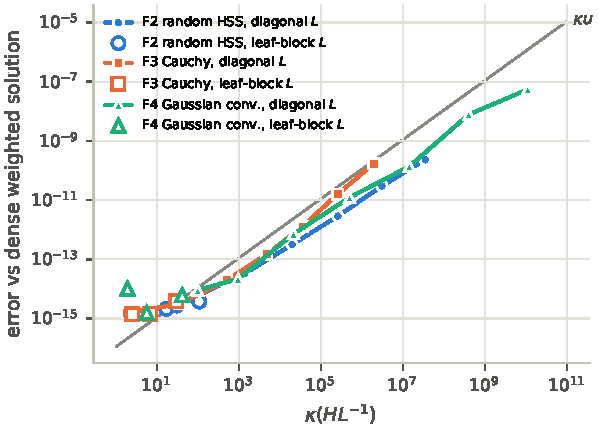
\includegraphics[width=0.55\textwidth]{figures/m2_weighted.pdf}
\caption{W1: weighted minimum-norm error against $\kappa(HL^{-1})$. Filled: diagonal $L$ with up to
12 decades of dynamic range. Open: leaf-block SPD $L$. Grey: $\kappa u$.}
\label{fig:W}
\end{figure}

\subsection{Tikhonov}\label{subsec:Tnum}
\textbf{T1 (accuracy along the $\lambda$ path).} $\lambda/\|H\|_2=10^{-8},\dots,10^{2}$ for wide
($1024\times2048$), square ($1536^2$) and tall ($2048\times1024$) F2, for the wide stride-2 ``valid''
Gaussian convolution ($1016\times2048$, F4) and for a square stride-1 ``same'' Gaussian convolution
($1536^2$). The reference is the dense SVD filter solution
$\sum_i\frac{\sigma_i}{\sigma_i^2+\lambda^2}(u_i^*b)v_i$. Figure~\ref{fig:T}a: errors of
$4\times10^{-15}$--$4\times10^{-13}$ for the F2 matrices and the wide convolution at every $\lambda$,
including the tall case, where plain min-norm does not apply. For the tall case $\kappa(H_a)u$ is a
loose bound: at $\lambda=10^{-8}\|H\|$ it is $10^{-8}$, the error $4\times10^{-13}$
(Sec.~\ref{sec:tikhonov}). For the square convolution ($\kappa=2.4\times10^7$) the error at small $\lambda$
is $5\times10^{-10}$, below $\kappa(H_a)u=2.6\times10^{-9}$, and it falls to $10^{-14}$ as $\lambda$ grows and
$\kappa(H_a)$ drops. At $\lambda=100\|H\|$ the relative error
of $x$ rises to $10^{-13}$: there $\|x\|\approx\|H\|\|s\|/\lambda$ is a small part of $z=(x,s)$. The general
form ($S$, $L$ diagonal with 2 decades each) matches a dense stacked least-squares solve to
$9\times10^{-13}$ ($\lambda=10^{-4}$) and $1.2\times10^{-14}$ ($\lambda=1$).

\textbf{T2/T3 (scale and cost).} Manufactured Tikhonov solutions ($x_\star=H^*z$,
$b=Hx_\star+\lambda^2z$, so $x_\lambda=x_\star$ exactly) with $\lambda=10^{-2}$: error
$1.5\times10^{-15}$ (wide, up to $n=2^{19}$) and $1.2\times10^{-15}$ (tall $m=2n$, up to $n=2^{18}$),
flat in $n$ (Figure~\ref{fig:T}c). The cost is linear (Figure~\ref{fig:T}b). A Tikhonov solve costs
$1.0$--$1.25\times$ a min-norm solve of the same wide $H$, up to $n=2^{19}$ (5.3\,s against 4.5\,s there).
That is below the factor $1+m/n=1.5$ one might expect from the wider leaves, because the size
reduction removes the extra columns at once (Sec.~\ref{sec:tikhonov}).

\begin{figure}[t]
\centering
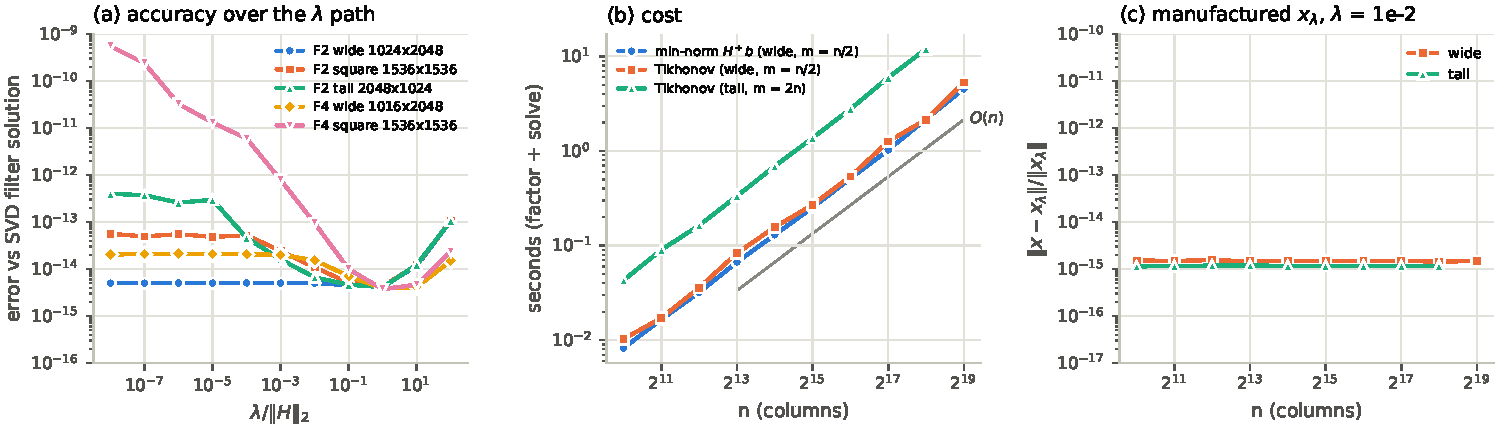
\includegraphics[width=\textwidth]{figures/m2_tikhonov.pdf}
\caption{T1--T3. (a) Error against the SVD filter solution along the $\lambda$ path. (b) Cost against
min-norm. (c) Manufactured Tikhonov solutions at scale.}
\label{fig:T}
\end{figure}

% ======================================================================
\section{Applications}\label{sec:apps}

\subsection{Basis pursuit: IRLS and Douglas--Rachford}\label{subsec:bp}
\emph{Problem.} Seismic reflectivity is modelled as a sparse spike train convolved with a band-pass
wavelet. $x_0\in\mathbb{R}^{4096}$ has 60 spikes (amplitudes $\pm[0.5,1.5]$, separation $\ge24$ samples).
$H$ is the Ricker wavelet ($\sigma=2.5$) convolution with stride 2, F4, $2038\times4096$, and
$b=Hx_0$. We solve basis pursuit, $\min\|x\|_1$ s.t.\ $Hx=b$, in two ways:
\begin{itemize}[leftmargin=1.4em,itemsep=1pt]
\item \textbf{IRLS} (Daubechies--DeVore--Fornasier--G\"unt\"urk~\cite{ddfg}). Repeat
$x^{k+1}=\operatorname*{arg\,min}_{Hx=b}\sum_jw_j^k|x_j|^2$ with $w_j^k=(|x_j^k|^2+\varepsilon_k^2)^{-1/2}$ and
$\varepsilon_{k+1}=\min(\varepsilon_k,|x^{k+1}|_{(s+1)}/n)$. \emph{The inner problem is exactly (W) with
$L=\operatorname{diag}(\sqrt{w^k})$.} The weights change every step, so each step is a fresh
factorization of $HL_k^{-1}$, and Theorem~\ref{thm:W} guarantees each inner solve is the exact
weighted minimum-norm point.
\item \textbf{Douglas--Rachford} on $\|x\|_1+\iota_{\{Hx=b\}}$:
$x^k=P(z^k)$, $z^{k+1}=z^k+\operatorname{soft}_\gamma(2x^k-z^k)-x^k$, $\gamma=0.05$, with the projection
$P(v)=v+H^+(b-Hv)$. Here $H$ never changes. It is factored \emph{once} and each step is one $O(nr)$
solve plus two HSS products. ADMM for the same problem has the same inner step.
\end{itemize}
\emph{Results} (Figure~\ref{fig:bp}). The minimum-norm solution has relative error 0.71: it is smooth,
not sparse. IRLS reaches $10^{-8}$ after 24 iterations and $1.6\times10^{-10}$ after about 33; DR reaches $8\times10^{-9}$ after 67.
One factorization costs 0.056\,s and one solve 0.0023\,s, so a DR step is $\approx24\times$ cheaper than
an IRLS step, and DR wins in wall time (0.25\,s against 1.5\,s to $10^{-8}$). The legacy MATLAB solver
refactors on every call, so with it DR loses that advantage. In the current code $H$ keeps its factors,
so the projection \texttt{v + H\textbackslash(b - H*v)} factors only on the first call.

\begin{figure}[t]
\centering
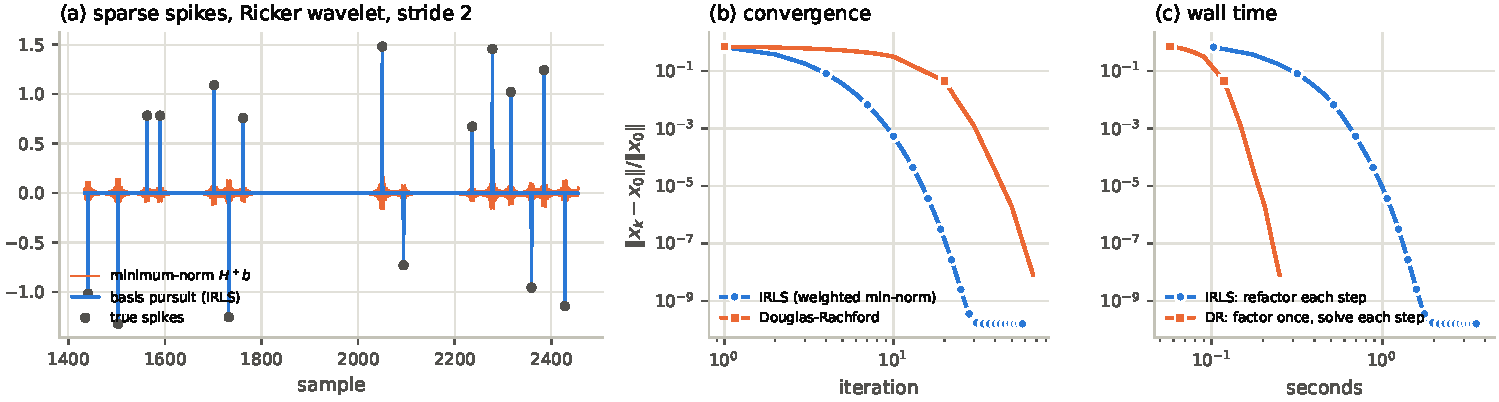
\includegraphics[width=\textwidth]{figures/m2_bp.pdf}
\caption{Basis pursuit for sparse-spike deconvolution. (a) Detail of the recovered spike train.
(b, c) Convergence in iterations and in wall time.}
\label{fig:bp}
\end{figure}

\subsection{Tikhonov deblurring and the choice of $\lambda$}\label{subsec:db}
The signal of M1, Sec.~\ref{M1-subsec:a2} ($n=4096$), Gaussian blur $\sigma=3$, stride 2, 1\% white noise.
The minimum-norm solution has error 94: it inverts the noise. A sweep of 23 values of $\lambda$ costs
0.07\,s per $\lambda$ (one factorization each). The discrepancy principle (largest $\lambda$ with
$\|Hx_\lambda-b\|\le1.01\|e\|$) gives $\lambda=0.32$ with error 0.046, against the best on the grid,
0.036 at $\lambda=0.56$ (Figure~\ref{fig:db}). The L-curve corner (maximum curvature) is at
$\lambda=0.032$, ten times smaller, with error 0.30: here the L-curve under-regularizes, a known
limitation for smooth solutions~\cite{hanke}. The discrepancy principle needs $\|e\|$, which this test
knows.

\begin{figure}[t]
\centering
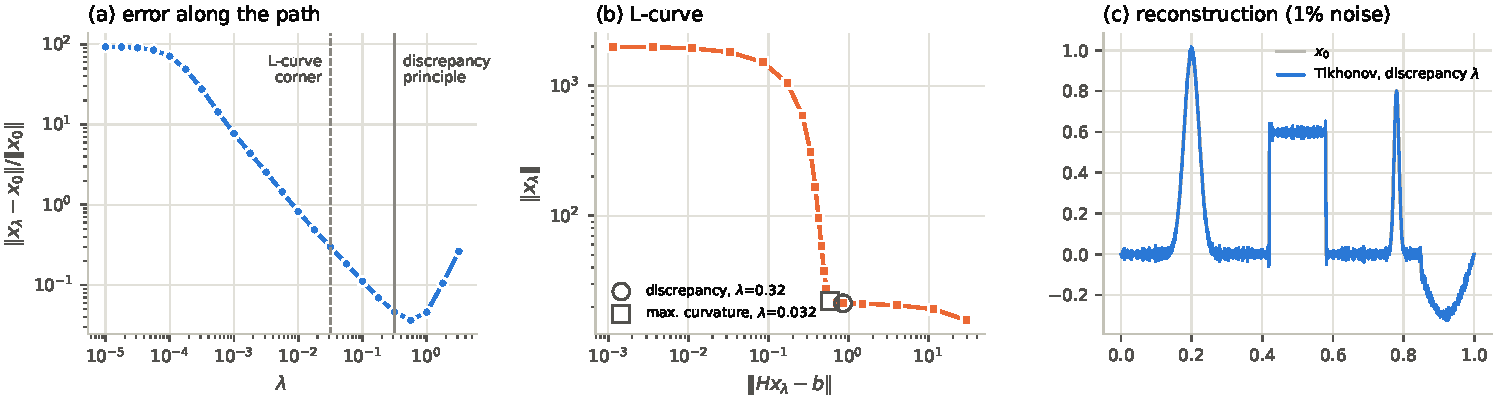
\includegraphics[width=\textwidth]{figures/m2_deblur.pdf}
\caption{Tikhonov deblurring: error along the path, L-curve (circle: discrepancy principle, square:
maximum curvature), and the discrepancy-principle reconstruction.}
\label{fig:db}
\end{figure}

\subsection{Non-Cartesian MRI with $k$-space weights}\label{subsec:mri}
\emph{Problem} (1-D model). Image $x_0$ on a centred grid of $N=2048$ pixels (piecewise constant plus a
bump). Data are $m=921$ samples of its Fourier transform at variable-density non-Cartesian
frequencies $\xi_j$, denser near $k=0$. With $x'_j=-\xi_j\bmod1$ this is exactly F5, with the
Cartesian $k$-space grid $l/N$ as the HSS column coordinates and $y=Fx$ as the unknown. A diagonal
weight on $y$ is therefore leaf-diagonal: the case this memo covers. The weight is
$L=\operatorname{diag}(1+|k_l|/k_0)$, i.e.\ the Gaussian prior with power spectrum $(1+|k|/k_0)^{-2}$
appropriate for piecewise-smooth images.

\emph{Results} (Figure~\ref{fig:mri}). Exact data: the image error is 0.120 for minimum norm and 0.098
for the weighted solution at $k_0=8$. The optimum over $k_0\in\{1,\dots,64\}$ is shallow, between 0.098
and 0.105. With 2\% noise the unweighted minimum-norm image is useless (error $2\times10^{7}$): the
variable-density nodes make $C$ severely ill-conditioned. Weighted Tikhonov at $\lambda=0.1$ restores
an error of 0.24. \emph{Tree.} Variable density is where the constructor's index-based split hurts most:
maximum HSS rank 135 with it, against 36 with the geometry-aligned tree (\texttt{mp\_tree\_aligned}).

\begin{figure}[t]
\centering
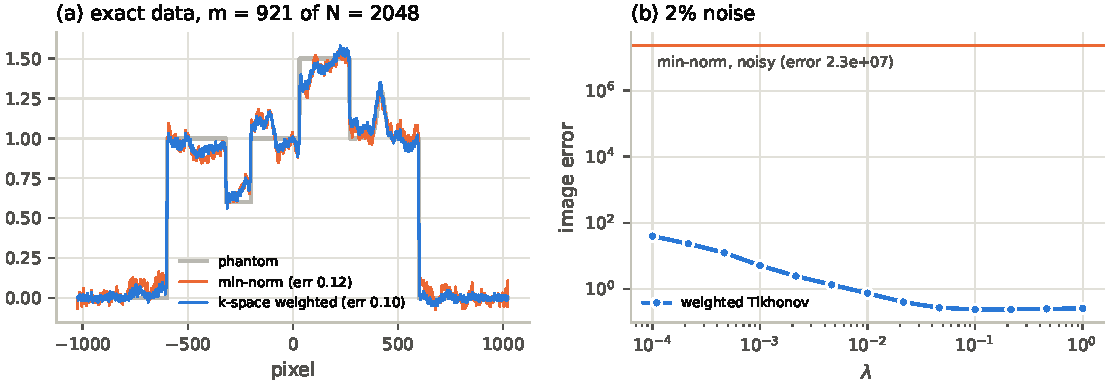
\includegraphics[width=0.85\textwidth]{figures/m2_mri.pdf}
\caption{1-D non-Cartesian MRI. (a) Exact data: minimum norm against $k$-space-weighted minimum norm.
(b) 2\% noise: weighted Tikhonov along the path against the unregularised minimum-norm image.}
\label{fig:mri}
\end{figure}

\subsection{Where the weights are not diagonal}\label{subsec:notdiag}
Two items from the list need weights that this memo does not cover (Remark~\ref{rem:nonconform}):
\begin{itemize}[leftmargin=1.4em,itemsep=1pt]
\item \emph{Seismic MWNI}: the HSS coordinates are the regular \emph{spatial} grid, but the weights live
on wavenumbers, so $L=F^*\operatorname{diag}(P^{-1/2})F$ is circulant.
\item \emph{Image-domain sparsity in MRI} (compressed sensing): the HSS coordinates are $k$-space, but the
IRLS weights live on pixels, which is again circulant.
\end{itemize}
Both are covered once $L$ is allowed to be an HSS matrix (circulants with smooth symbols are). That
needs HSS inversion and HSS products, which the repo does not have yet: the natural next step.
Alternatively, ADMM can split the weight off into its own step; then only the unweighted
minimum-norm solve is needed, in the HSS coordinates.


\section{Open Items}\label{sec:open2}
\begin{enumerate}[leftmargin=1.5em,itemsep=2pt]
\item \textbf{Factor/solve split}: done. $H$ keeps its factors after the first solve, and \texttt{minnorm} and
\texttt{tikhonov} keep theirs for the last weight and the last $(\lambda,L,S)$ (M1, Sec.~\ref{M1-sec:open}). Douglas--Rachford
and ADMM need many solves with one matrix, and with stored factors a solve is $\approx24\times$ cheaper than
a factorization in the basis-pursuit test (Section~\ref{subsec:bp}) and $4$--$16\times$ at the sizes of M1,
Table~\ref{M1-tab:scaling}. A Tikhonov $\lambda$ sweep still needs a new factorization per $\lambda$.
A factorization that reuses the $\lambda$-independent parts (the $U$-compressions are the same
for every $\lambda$) would cut that, and is worth working out.
\item \textbf{HSS weights.} Circulant or smoothing weights (MWNI, image-domain sparsity) need $L$ itself
HSS, and with it HSS inversion and products (Remark~\ref{rem:nonconform}).
\item \textbf{General-form Tikhonov with a difference operator} ($L$ a non-square
$(n-1)\times n$ first difference) is not covered by the substitution. It needs the
$A$-weighted pseudo-inverse (Eld\'en's standard-form transformation) or a stacked formulation
with an extra block row.
\item \textbf{Geometric tree} for variable-density sampling (rank 135 against 36 here; M1,
Sec.~\ref{M1-sec:open}).
\end{enumerate}

\appendix
\section{Code}
\sloppy
MATLAB methods of \texttt{@hss}: \texttt{x = minnorm(H,b,'Weight',L)} and
\texttt{[x,r] = tikhonov(H,b,lambda,'Weight',L,'DataWeight',S)}, where $L$ and $S$ are vectors (diagonal)
or cell arrays of leaf blocks; omitted means identity. Both keep their factors with $H$ (a repeat call with
the same weights and $\lambda$ only solves). Generator edits in \texttt{@hss/private/}: \texttt{hss\_to\_gen},
\texttt{hss\_from\_gen}, \texttt{hss\_gen\_weight} (leaf blocks applied by solves, never by \texttt{inv}),
\texttt{hss\_gen\_augment}. The suite's \texttt{mp\_weighted\_minnorm} and \texttt{mp\_tikhonov} are thin
wrappers. Tests: \texttt{mp\_selftest}, \texttt{mp\_test\_solver} and \texttt{test\_hss.m} (leaf-block weights
against dense formulas), \texttt{mp\_exp\_weighted\_tikhonov}, \texttt{mp\_exp\_apps2}. Python: \texttt{hssmn.variants}
(\texttt{weighted\_minnorm}, \texttt{tikhonov}, \texttt{augment}); experiments \texttt{exp\_w\_t.py},
\texttt{exp\_apps2.py}; figures \texttt{fig\_memo2.py}.

\begin{thebibliography}{9}\small
\bibitem{memo1} A.~Sethi-Olowin, \emph{The recursive complete minimum-norm HSS solver: proofs,
numerical experiments, and applications}, memo, October 2026 (cited as M1).
\bibitem{ddfg} I.~Daubechies, R.~DeVore, M.~Fornasier, C.~S.~G\"unt\"urk, Iteratively reweighted least
squares minimization for sparse recovery, \emph{Comm. Pure Appl. Math.} 63 (2010).
\bibitem{lsqr} C.~C.~Paige, M.~A.~Saunders, LSQR: an algorithm for sparse linear equations and sparse
least squares, \emph{ACM TOMS} 8 (1982).
\bibitem{mwni} B.~Liu, M.~D.~Sacchi, Minimum weighted norm interpolation of seismic records,
\emph{Geophysics} 69 (2004).
\bibitem{elden} L.~Eld\'en, A weighted pseudoinverse, generalized singular values, and constrained
least squares problems, \emph{BIT} 22 (1982).
\bibitem{hansen} P.~C.~Hansen, \emph{Rank-Deficient and Discrete Ill-Posed Problems}, SIAM, 1998.
\bibitem{hanke} M.~Hanke, Limitations of the L-curve method in ill-posed problems, \emph{BIT} 36 (1996).
\end{thebibliography}
\end{document}
